\section{Introduction}
\begin{frame}{Origins of Algebra}
    \begin{itemize}
      \item \textbf{Mesopotamia \& Egypt (c. 2000–1600 BCE)}
        \begin{itemize}
          \item Early problem-solving (linear/quadratic equations) in word problems
          \item No formal symbols, but systematic procedures
        \end{itemize}
  
      \item \textbf{Greek Era (c. 600 BCE–300 CE)}
        \begin{itemize}
          \item Geometric methods for solving equations (Euclid, Apollonius)
          \item Diophantus introduced proto-symbolic notation
        \end{itemize}
  
      \item \textbf{Islamic Golden Age (8th–12th Century)}
        \begin{itemize}
          \item Al-Khwarizmi’s work \emph{Al-jabr} $\rightarrow$ term “Algebra”
          \item Systematic solutions for linear and quadratic equations
        \end{itemize}
  
      \item \textbf{Transmission to Europe (12th–17th Century)}
        \begin{itemize}
          \item Latin translations influenced Fibonacci, others
          \item Viète, Descartes established modern symbolic notation \& analytic geometry
        \end{itemize}
  
      \item \textbf{Modern Algebra (19th–20th Century)}
        \begin{itemize}
          \item Emergence of abstract algebra (groups, rings, fields)
          \item Galois, Abel, and others formalized algebraic structures
        \end{itemize}
    \end{itemize}
  \end{frame}
  \begin{frame}{What is Algebra?}
    Algebra is a branch of mathematics that deals with numbers, variables, and their relationships. Key concepts include:
    \begin{itemize}
        \item \textbf{Variables}: Symbols (like \( x \), \( y \)) representing unknown or changing values.
        \item \textbf{Expressions}: Combinations of variables, numbers, and operations. E.g., \( 2x + 3 \).
        \item \textbf{Equations}: Mathematical statements that express equality, e.g., \( 2x + 3 = 7 \).
        \item \textbf{Solving Equations}: Finding values for variables that make an equation true.
        \item \textbf{Polynomials}: Expressions like \( 3x^2 + 2x - 5 \) involving variables raised to powers.
        \item \textbf{Functions}: Describes a relationship between variables, e.g., \( y = 2x + 1 \).
    \end{itemize}
\end{frame}
\begin{frame}{Why Algebra is Important in Machine Learning}
 
    \begin{itemize}
      \item \textbf{Data Representation:}  
      Data is often represented as vectors, matrices, and tensors. Algebra provides the tools for efficiently handling these structures.
      \item \textbf{Model Building:}  
      Many machine learning models (e.g., linear regression, neural networks) rely on algebraic operations like matrix multiplication and linear transformations.
      \item \textbf{Optimization:}  
      Training models involves solving systems of equations, computing gradients, and performing matrix decompositions, all of which require algebra.
      \item \textbf{Theoretical Insights:}  
      Concepts such as feature spaces, eigenvalues, eigenvectors, and dimensionality reduction (e.g., PCA) are based on algebraic principles.
      \item \textbf{Computational Efficiency:}  
      Algebraic methods enable the development of efficient algorithms that can be optimized for modern hardware.
    \end{itemize}
 
\end{frame}


  \begin{frame}{Integers}
    \begin{itemize}
        \item The set of integers is denoted by \(\mathbb{Z}\).
        \item Integers include:
        \[
          \ldots, -3, -2, -1, 0, 1, 2, 3, \ldots
        \]
        \item Formally, \(\mathbb{Z} = \{\dots, -2, -1, 0, 1, 2, \dots\}\).
        \item Common properties:
        \begin{itemize}
            \item \(\mathbb{Z}\) is infinite and unbounded in both the negative and positive directions.
            \item Closed under addition, subtraction, and multiplication:
                \[
                  \forall a, b \in \mathbb{Z}, \quad
                  a \pm b \in \mathbb{Z}, \quad
                  a \cdot b \in \mathbb{Z}.
                \]
        \end{itemize}
        \item The quotient of any two integers is not necessarily an integer. So we need to extend arithmetic to \textbf{rational numbers}
    \end{itemize}
\end{frame}
% Slide: Rational Numbers
\begin{frame}{Rational Numbers}
    \begin{itemize}
        \item The set of rational numbers is denoted by \(\mathbb{Q}\).
        \item Definition:
        \[
          \mathbb{Q} = \left\{ \frac{p}{q} \,\middle|\,
            p \in \mathbb{Z}, \; q \in \mathbb{Z}, \; q \neq 0
          \right\}.
        \]
        \item Every integer is also a rational number (e.g., \(5 = \frac{5}{1}\)).
        \item Examples:
        \[
          \frac{1}{2}, \quad -\frac{3}{4}, \quad 0, \quad 7, \quad \frac{11}{5}, \ldots
        \]
        \item Properties:
        \begin{itemize}
            \item Closed under addition, subtraction, multiplication, and division (except division by zero).
            \item Densely packed on the number line: between any two rationals, there is another rational.
        \end{itemize}
    \end{itemize}
\end{frame}
\begin{frame}
    \frametitle{Interesting Facts}
    \begin{itemize} 
        \item Why division by zero is prohibited ?
        \begin{itemize}
            \item Division is inverse of multiplication in the sense  
            \[  
            \frac{m}{n} \cdot n = m
            \]
        \item if \( n=0 \) and \( m = 1\), we get \(\frac{1}{0} \cdot 0 = 1\) which is nonsensical as any number multiplied by zero is zero
        \end{itemize}
        \item Rational numbers suffice for all actual physical measurements like weight, height and length
        \item But Geometry, Algebra and Calculus force us to consider \textbf{real numbers}
    \end{itemize}
\end{frame}
\begin{frame}
    \frametitle{A Real Number Line}
    \begin{figure}[h]    
        \begin{minipage}[b]{0.8\textwidth}
        \centering
        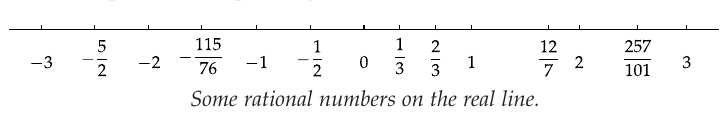
\includegraphics[scale=0.35]{real-line.png}
    \end{minipage}
\end{figure}
\begin{itemize}
    \item if \( n\) is a positive integer then \( \frac{1}{n}\) is to the right of 0 by the length obtained by dividing the segment from \( 1 to 0\) in to \( n \) segments of equal length
\end{itemize}
\end{frame}
\begin{frame}
    \frametitle{Is every Real Number a Rational}
    \begin{figure}[h]    
        \begin{minipage}[b]{0.8\textwidth}
        \centering
        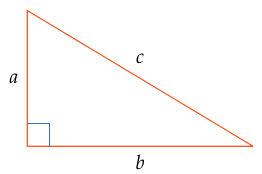
\includegraphics[scale=0.35]{irrational-geometry.png}
        \end{minipage}
    \end{figure}
    \begin{itemize}
        \item \( c^{2} = a^{2} + b^{2} \). If \( a = 1, b = 1\) then \(c^{2} = 2 \). Then what rational number is \( c \)
        \item By trial and error, \( c = \left( \frac{99}{70} \right)^{2}  = \frac{9801}{4900}\) where the numerator just misses twice the denominator by 1. But this is not 2 but close to 2. Another number is \( \left( \frac{9369319}{6625109} \right)^{2} = 1.999999999999977\) , but not 2
        \item Greeks proved that it is impossible to find any rational number whose square is 2
    \end{itemize} 
\end{frame}
\begin{frame}
    \frametitle{Proof: No rational number has a square equal to 2}
    Let m and n are two integers
    \[ 
        \left( \frac{m}{n} \right)^{2} = 2  
    \]
    By canceling any common factors, m and n are reduces to its lowest terms 

    \[
         m^{2} = 2n^{2}
    \]

    this makes \(m^{2}\) even, hence \(m\) is an even. (The square of even is even and odd is odd). So \(m = 2k\) for some integer \(k\)

    Substituting \(m = 2k\) in the equation gives, \(4k^{2} = 2n^{2} \), which results in 
    \[
        2k^{2} = n^{2}
    \]
    which means \( n^{2}\) is even and therefore \(n \) is even
    \\
    \(\frac{m}{n} \) has common factors which contradicts the earlier assumption
\end{frame}
\begin{frame}
    \frametitle{Irrational Number}

    \begin{block}{Irrational Number}
        A real number that is not rational is \textbf{irrational number}
    \end{block}
    \begin{itemize}
        \item \( \sqrt(2)\)
        \item \(3+\sqrt(2)\)
        \item \(8\sqrt(2)\)
    \end{itemize}
\end{frame}